% Inoffizielle LaTeX-Vorlage für Bachelor-/Masterarbeiten
% an der Fakultät für Chemie und Pharmazie
% der Albert-Ludwigs-Universität Freiburg
%
% Diese Vorlage ist lediglich ein Vorschlag, der versucht, sowohl
% typografischen Ansprüchen ansatzweise gerecht zu werden als auch
% nutzbar zu sein.
%
% Jegliche Nutzung auf eigene Verantwortung.
%
% Copyright (c) 2018, Till Biskup

\chapter{Ergebnisse und Diskussion}
\label{ch:ergebnisse_diskussion}

Ergebnisse und Diskussion können in zwei separate, aufeinander folgende Kapitel aufgeteilt werden. Die eigene Erfahrung spricht allerdings eher dagegen.

Werden Ergebnisse und Diskussion, wie hier vorgegeben, in einem Kapitel gemeinsam abgehandelt, ist es umso wichtiger darauf zu achten, dass zunächst die eigentlichen Ergebnisse beschrieben und dann erst im Kontext anderer Arbeiten diskutiert werden. Eine reine Darstellung der Ergebnisse in Abbildungen und Tabellen ist \emph{nicht} ausreichend.

Auch die -- für gewöhnlich in Tabellen übersichtlich aufbereiteten -- Parameter von Simulationen, die an gemessene Daten angepasst wurden, gehören \foreign{per se} erst einmal zu den Daten, die textlich beschrieben werden sollten.



\section{Umgang mit Abbildungen}

Abbildungen sollten nach Möglichkeit immer als vektorisierte Grafikformate vorliegen. Die Erfahrung zeigt, dass es möglich ist, Abbildungen von Anfang an so anzulegen, dass sie sowohl in der Abschlussarbeit als auch in einem zugehörigen Vortrag verwendet werden können. Die zur Beschriftung von Abbildungen verwendete Schriftgröße ist für beide Fälle passend.

Wer diesen Ansatz verfolgt, kann ggf. das Abbildungsverzeichnis auf eine Ebene mit der Abschlussarbeit und dem Vortrag verschieben und die relativen Pfade in der Präambel-Datei zur Handhabung von Abbildungen (\filename{grafiken.tex}, vgl. Listing~\ref{lst:grafiken}, S.~\pageref{lst:grafiken}) entsprechend anpassen.

Das Verzeichnis für die Abbildungen ist weiter unterteilt in eigene und fremde Abbildungen. Für fremde Abbildungen ist es eine gute Idee, in einer Datei mit gleichem Grundnamen (und evtl. der Endung \filename{.txt}) Hinweise zum jeweiligen Urheberrecht abzulegen, die sich dann ggf. in die Abbildungsunterschrift übernehmen lassen.

Dieses Dokument ist von seinem Layout so angelegt, dass als Breite des Satzspiegels\footnote{Als Satzspiegel oder Schriftspiegel wird die nutzbare Fläche einer Buchseite bzw. allgemein einer Textseite eines gedruckten Dokuments bezeichnet.} recht genau 15~cm entspricht. Werden die Abbildungen entsprechend im Format 15:10 oder 15:9 angelegt, lassen sie sich unskaliert direkt in dieses Dokument einbinden und auf Seitenbreite skaliert in eine Vortragsfolie (bei Verwendung des Layouts der Albert-Ludwigs-Universität Freiburg und des \package{beamer}-Pakets für \LaTeX{}).

Wie schon für Tabellen in Kapitel~\ref{ch:material_methoden} angesprochen, haben Abbildungen, auf die aus dem Text nicht verwiesen wird, keine Daseinsberechtigung. Entsprechend sei hier auf Abb.~\ref{fig:beispiel} verwiesen.

\begin{figure}[t]
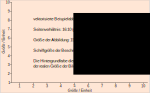
\includegraphics{Beispielabbildung}
\caption[Abbildungen haben immer eine Bildunterschrift.]{\textbf{Abbildungen haben immer eine Bildunterschrift.} Außerdem ist es hilfreich, wenn die Bildunterschrift die Abbildung soweit erklärt, dass der geneigte Leser nicht erst noch große Teile des Textes lesen muss, um sie zu verstehen. Kurz: Abbildungen sollten gemeinsam mit ihrer Unterschrift für sich stehen.}
\label{fig:beispiel}
\end{figure}
